\documentclass[11pt, aspectratio = 169]{beamer}
% aspectratio = 169, aspectratio=43

  \usepackage{graphicx}
  \usepackage[english]{babel}
%  \usepackage{parskip}
  \usepackage{amsmath}
  \usepackage{listings}
  \usepackage{amsfonts}
  \usepackage{mathtools}
  \usepackage{amssymb}
  \usepackage{booktabs}
  \usepackage{braket}
  \usepackage{amsthm}
  \usepackage{siunitx}
  \usepackage{bm}
  \usepackage[suftesi]{frontespizio}
  \usepackage{color}
  \usepackage{newfloat}
  \usepackage{wrapfig}
  \usepackage{tikz}
  \usepackage{pgfplots}
  \usetikzlibrary{patterns}
  \usepackage{comment}
  \usepackage{mathrsfs}
  \usepackage{epstopdf}
%  \usepackage{hyperref}
  \usepackage[normalem]{ulem}

  \usepackage{media9}
  \usepackage{multimedia}
  %\usepackage[T1]{fontenc}
  %\usepackage{mathptmx}

\newcommand<>{\alertb}[1]{\begingroup%
\setbeamercolor{alerted text}{fg=blue!80!white}\alert{#1}\endgroup}

\NewDocumentCommand{\reff}{s m}{%
  \IfBooleanTF{#1}% Check for starred variant
    {\beamer@origref{#2}}% \reff*
    {\hyperlink{#2}{\beamer@origref{#2}}}% \reff
}

  \newcommand{\pt}{\,\, .}
  \newcommand{\cm}{\,\, ,}
  \newcommand{\pc}{\,\, ;}
  \newcommand{\be}[1]{\begin{equation}
	  \label{#1}}
  %\newcommand{\lb}[1]{\label{#1}}
  \newcommand{\ee}{\end{equation}}

  \def\ba#1#2\ea{\begin{align}\label{#1}#2\end{align}}

  %\def\bfr#1#2\efr{\begin{frame}\frametitle{#1}#2\end{frame}}
  \newcommand{\bfr}[1]{\begin{frame}
          \frametitle{#1}}
  %\newcommand{\lb}[1]{\label{#1}}
  \newcommand{\efr}{\end{frame}}

  \title[Thesis]{\textbf{Out-of-equilibrium dynamics in
round-trip and dissipation protocols} }
  \author[F.Tarantelli]{Francesco Tarantelli  \\ 
  \texttt{francesco.tarantelli@phd.unipi.it}}
  \date[ ]{$17^{\rm th}$ January}
  \institute[unipi]{University of Pisa and INFN}
  \logo{\textcolor{white!50!red}{\small \texttt{PhD}}}
  %\logo{\includegraphics[width=15mm]{slides/figs/logo-white.pdf}} % logo.eps   -black   -white
  
  \usetheme{Berkeley}%[width=2.2cm]
  
  %\useoutertheme[left, height=0pt, width=4cm]{sidebar}
  %\setbeamerfont{title in sidebar}{size}
  %\setbeamerfont{sidebar}{size=\scriptsize}
  %\setbeamerfont{section in sidebar}{size=\small}
  %\setbeamerfont{sidebar}{size=\large}%\scriptsize}
%  \useoutertheme[left]{sidebar}

  \setbeamercovered{dynamic}
%%%%%%%%%%%%%%%%%%%%%%%%%%%%%%%%%%%%%%%%%%%%%%%%%%%%%%%%%%%%%%%%%%%%%%%%%%%%%%%%%%%%%%%%%%%%%%%%%%%%%
  %\usecolortheme{seahorse}
%%

\setbeamercolor*{logo}{fg=white,bg=black!50!cyan}

\setbeamercolor*{structure}{fg=black!70!blue}
\setbeamercolor*{title}{fg=black!80!white,bg=black!20!cyan}
%\setbeamercolor*{block title}{bg=blue!90!black,fg=blue}
%\setbeamercolor*{block title example}{bg=cyan!90!black,fg=white}
%\setbeamercolor*{block title example}{fg=black,bg=orange}
\setbeamercolor*{alerted text}{fg=red!30!black}

%\setbeamercolor*{palette primary}{bg=black,fg=white}
%\setbeamercolor*{palette secondary}{bg=blue!75!black,fg=blue}
%\setbeamercolor*{palette tertiary}{bg=green!50!black!,fg=blue} %title in head/foot   %title in sidebar

\setbeamercolor*{frametitle}{bg=black!10!cyan,fg=white}
\setbeamercolor*{framesubtitle}{fg=white!80!cyan}

\setbeamercolor*{sidebar}{bg=black!10!cyan}

\setbeamercolor*{title in sidebar}{fg=black!100!white}
\setbeamercolor*{author in sidebar}{fg=white}
\setbeamercolor*{section in sidebar shaded}{fg=black!100!cyan}
\setbeamercolor*{section in sidebar}{bg=black!100!cyan,fg=black!20!cyan}
\setbeamercolor*{subsection in sidebar shaded}{fg=white!100!cyan}
\setbeamercolor*{subsection in sidebar}{bg=white!80!cyan,fg=black!90!cyan}

%%%%%%%%%%%%%%%%%%%%%%%%%%%%%%%%%%%%%%%%%%%%%%%%%%%%%%%%%%%%%%%%%%%%%%%%%%%%%%%%%%%%%%%%%%%%%%%%%%%%%

%  \setbeamertemplate{sections/subsections in toc}[ball]%[circle]%
  \setbeamertemplate{items}[circle]

  \theoremstyle{definition}

  \theoremstyle{plain}

  \newcommand{\numberset}{\mathbb}
  \newcommand{\C}{\numberset{C}}
  \newcommand{\R}{\numberset{R}}
  \newcommand{\N}{\numberset{N}}
  \newcommand{\Z}{\numberset{Z}}
  \newcommand{\D}{\numberset{D}}

%  \renewcommand{\vec}{\bm}


  \DeclarePairedDelimiter{\norma}{\lVert}{\rVert}
  \DeclarePairedDelimiter{\abs}{\lvert}{\rvert}

  \setbeamertemplate{caption}[numbered]

  %*******************
  % IMPORTANT:
  %*******************
  \usefonttheme[onlymath]{serif} 
  %*******************

\beamertemplatenavigationsymbolsempty
%\setbeamertemplate{footline}[frame number]

\addtobeamertemplate{navigation symbols}
{\tiny %
    \usebeamerfont{footline}%
    \usebeamercolor[fg]{footline}%
    \hspace{1em}%
    \insertframenumber/\inserttotalframenumber
}

\setbeamercolor{navigation symbols}{fg=black}

\begin{document}

   \begin{frame}
      \frametitle{PhD Discussion}
      \maketitle
      
      \begin{tikzpicture}[remember picture,overlay]
           \node [shift={(-13cm, -7.6cm)}] at (current page.north east)
           {\includegraphics[width=2cm]{slides/figs/logo.pdf}}; 
      \end{tikzpicture} 
      
      \begin{tikzpicture}[remember picture,overlay] 
           \node [shift={(-1.5cm, -7.6cm)}] at (current page.north east) 
           {
\includegraphics[width=3cm]{slides/figs/logoinfnp.pdf}}; 
      \end{tikzpicture}
      
   \end{frame}


%   \begin{frame}
%      \frametitle{Presentation plan}
%      \tableofcontents
%   \end{frame}

   \chapter{Introduction}









\subsubsection{Outline}


for the chapter 2 we use the Quantum Ising Model as paradigmatic model, while in the third
one, we adopt the lattice Kitaev model. The choice is justified by the fact that for an 
unitary time-evolution is sufficient to know the wave function $\ket \psi$, instead in 
the case of a dissipation process, it is necessary to consider the density matrix $\rho$.

The Kitaev model is quadratic in its site operator, therefore the complexity of the 
diagonalization scales linearity with the system size. In the other hand, for the 
Quantum Ising model in the presence of longitudinal magnetization, the diagonalization
problem is exponentially complex. For these computational arguments, we could motivate
our toy model choices.


   \begin{comment}

\section{Paradigmatic Models}
	\subsection[Classical]{Classical Model}

\begin{frame}
	\frametitle{Classical Ising Model}
	
	2D Classical Ising Hamiltonian with size $L$x$L$ and with PBC:
	\begin{columns}
		\begin{column}{0.5\textwidth}
		
		
\begin{figure}[!h]
		\centering
		\begin{tikzpicture}
			\begin{axis} [width=8cm,height=3.2cm,xmax=1, axis lines=middle, 
			enlargelimits,
			xtick={0.5},ytick={0.},xticklabels={$T_c$},yticklabels={$ $}, 
			xlabel=$T$,ylabel=$w$]
				\draw [dashed, line width=0.5pt,gray] (50,-60) -- (50,60);
				\node[text=blue] at (30,7) {\scriptsize{$M>0$}};
				\node[text=blue] at (30,-8) {\scriptsize{$M<0$}};
				\node[text=red] at (70,7) {\scriptsize{$M=0$}};
				\node[text=red] at (70,-8) {\scriptsize{$M=0$}};
				\node[text=red] at (70,-8) {\scriptsize{$M=0$}};
				\addplot [domain=0:0.5, samples=10,smooth,thick,black] {0};
				\filldraw [red] (49,-0.7) rectangle ++(3pt,3pt); %circle (3pt)
			\end{axis}
		\end{tikzpicture}
	\end{figure}			
	
		\end{column}
		\begin{column}{0.5\textwidth}
		
	\begin{align} % \vec
		H_{\rm cl} = - J\,\sum_{\braket{i,\,\,j}}  &
		S_i \cdot  S_j -  w \cdot \sum _i  S_i  \,\,,\\
		Z = \sum _{\{S_i\}} &\, e^{-H/T}  \,\,;
	\end{align}			
	
		\end{column}
	\end{columns}
	
	\bigskip
	
	\alert{\bf Continuous Transition point:} 
	at $w = 0$ and $T_c =  \frac{2}{\ln(1+\sqrt{2})}\,\,(J=1\,\,{\rm fixed})$\\
	$ $\\
	\alert{RG dimensions}:	
	\begin{align}
		w \longrightarrow y_w = 15/8 \qquad 
		T \longrightarrow y_t =  1	\qquad
		{\rm Metropolis \,\,time}\,\,t \longrightarrow z = 2.1667(5) \,\,.\notag
	\end{align}
\end{frame}


	\subsection[Quantum]{Quantum Models}


\begin{frame}
	\frametitle{Quantum Ising Model}
	
	1D Quantum Ising Hamiltonian for a chain of size $L\,$ and PBC 
	($\hat \sigma_{L+1}^{(k)} = \hat \sigma_1^{(k)}$):
	\begin{align}
		\hat H_{\rm Is} = -\sum_{x=1}^{L} \hat \sigma^{(1)}_x \hat
  		\sigma^{(1)}_{x+1} - g\, \sum_{x=1}^L \hat \sigma^{(3)}_x 
  		- w \sum_{x=1}^L \hat \sigma_x^{(1)}\,\,;
	\end{align}
	$\sigma^{(k)} _x$ are the Pauli matrices on the $x^{\rm th}$ site in the
	$k$-axis direction.
	
	\bigskip
	\bigskip
	
	\alert{\bf Continuous Transition point:} 
	at $w = 0$ and $g_c = 1$\\
	\alert{RG dimensions}:	
	$ $\\
	\begin{align}
		w \longrightarrow y_w = 15/8 \quad 
		& r = g-g_c \longrightarrow y_r =  1	\quad
		{\rm  time}\,\,t \longrightarrow z = 1 \\
		&\hat \sigma _x^{(1)} \longrightarrow y_l = d + z - y_h = 1/8\,\,.\notag
	\end{align}
	
\end{frame}
\end{comment}

%\section{Kitaev model}
\begin{frame}
	\frametitle{Kitaev Model}
	Kitaev Hamiltonian mapped into a spin-$1/2$ XY chain, by a 
	Jordan-Wigner transformation (OBC):
	$\qquad \qquad\alert{\hat c \longrightarrow \hat\sigma}\,$
	\begin{align}
		\label{KitaevH}
		\hat H _K^{\rm (ABC)} =- \sum _{x=1}^{L}\biggr[ \bigl(
		 \hat c_x^\dagger \, \hat c_{x+1} + 
		 \hat c_{x+1}^\dagger \,\hat c_x \bigl) + 
		 \delta\,\bigl( \hat c_x \, \hat c_{x+1} + 
		\hat c_{x+1}^\dagger \, \hat c_x^\dagger \bigl)\biggr] - 
		\sum _{x=1}^L  \mu \, \hat c_x^\dagger \, \hat c_{x}  \,\,;
	\end{align}
	\begin{figure}[!h]
		\centering
		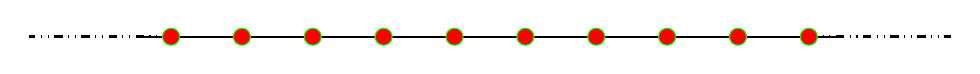
\begin{tikzpicture}[scale=0.9]
			\draw [-, line width=0.8pt, black] (-5.5,0.5) -- (4.5,0.5);

			\draw [dash dot dot, line width=1.2pt, black] (-5,0.5) -- (-7,0.5);
			\draw [dash dot dot, line width=1.2pt, black] (4,0.5) -- (6,0.5);

			\fill [red, draw=green] (-5,0.5) circle (0.12);
			\fill [red, draw=green] (-4,0.5) circle (0.12);
			\fill [red, draw=green] (-3,0.5) circle (0.12);
			\fill [red, draw=green] (-2,0.5) circle (0.12);
			\fill [red, draw=green] (-1,0.5) circle (0.12);
			\fill [red, draw=green] (4,0.5) circle (0.12);
			\fill [red, draw=green] (3,0.5) circle (0.12);
			\fill [red, draw=green] (2,0.5) circle (0.12);
			\fill [red, draw=green] (1,0.5) circle (0.12);
			\fill [red, draw=green] (0,0.5) circle (0.12);
			%\node (n) at (-4.5,0.85)  {$\bm{\hat c_1} $};
			%\node (n) at (4.5,0.95)  {$\bm{\hat c_L^\dagger} $};
		\end{tikzpicture}
	\end{figure}

	\alert{\bf Continuous Transition point:} 
	\begin{align}
		\mu _c = -2 \qquad {\rm and} \qquad \delta = 1 \,\,{\rm fixed} \,\,;\notag
	\end{align}
	\alert{RG dimensions}:	
	$ $\\
	\begin{align}
		w = \mu - \mu_c \longrightarrow y_w = 1 \qquad 
		\hat c_x \, ,\,\, \hat c_x^\dagger \longrightarrow y_c = 1/2 \qquad
		{\rm dynamic \,\, exp:\,\,} z =1
		\,\,.\notag
	\end{align}
	
\end{frame}

   \include{slides/model}
   \section{PART I}

\begin{frame}
	\frametitle{\Large{\rm PART I}}

\begin{center}
	{\LARGE{ \bf Round - Trip}\\}
	\medskip
	\medskip
	\medskip
	\texttt{ \Large
  FT, E. Vicari PR B {\bf 105}, 235124 \\ 
  FT, S. Scopa PR B {\bf 108}, 104316 }
\end{center}
\end{frame}

\section{KZ Protocol}

\begin{frame}
	\frametitle{Kibble Zurek(KZ) Protocol}
	\begin{itemize}
		\item[(i)] 
			Start at the equilibrium state (classical) and at the 
			\\ground state 
			$\ket{\Psi(t = t_i)} \equiv \ket{\Psi(w_i < 0 )}\,$ (quantum);
	\bigskip
	\bigskip
		
			\begin{columns}
				\begin{column}{0.4\textwidth}
			\item[(ii)] quantum case:
			\begin{align}
				\frac{ d \ket{ \Psi(t) } }{dt} = - i \hat H[w(t)] \ket{\Psi(t)} 
				\,\,; \notag
			\end{align}
				\end{column}
				\begin{column}{0.4\textwidth}
			\item[(ii)] classical one:	\\ $ $\\
			\alertb{\tt Metropolis algorithm};
				\end{column}
			\end{columns}
			\begin{align}
				& \alert{\Downarrow} \notag \\
				\alert{w(t)} &\alert{= t/t_s} \,\,; \notag
			\end{align}
			from $w_i < 0$ to $w_f > 0\,$, where $t_s$ is the time 
			scale of the slow variations of $w\,$.
	\bigskip
	\bigskip
	
		\item[(iii)] Then, for $t > t_f$, $w(t)$ decreases with the same
		  $t_s$ , from $w_f >0$ to the original value 
		 $wi < 0\,$, closing the cycle.
	\end{itemize}
\end{frame}

   \section{Observables}

\begin{frame}
	\frametitle{Observables}

	\begin{center}
	\alertb{\bf Classical Ising model}
	\begin{align}
		&M(t) = \frac{1}{L^2} \sum_{i} \braket{S_i}_t \,\,; \\
		&G(t,{\bm x},{\bm y}) \equiv \langle s_{\bm x}\, s_{\bm y}\,
		\rangle_t \,.
	\end{align}
	\end{center}
	\begin{center}
	\alertb{\bf Quantum models}\\
	Adiabaticity function:
	\begin{eqnarray}
  		A(t) = \Big|\braket{ \Psi_0[w(t)] | \Psi(t) }\Big|\,;
  		\label{adtfunc}
	\end{eqnarray}
	\end{center}
	
	%\begin{columns}
	%\begin{column}{0.5\textwidth}
	%\begin{center}
	%{\bf Ising:}
	%\begin{align}
	%	M(t) \equiv {1\over L} \sum_x  \langle \Psi(t) | \, \sigma_x^{(1)}
	%	| \Psi(t) \rangle\,;
	%	\notag
	%\end{align}
	%\end{center}
	%\end{column}
	%\begin{column}{0.4\textwidth}
	\begin{center}
	{\bf Kitaev:}
	\begin{align}
		C(x,t)  \equiv  \langle \Psi(t) |
  		\, c_j^\dagger c_{j+x} 
  		+ c_{j+x}^\dagger c_{j} \, | \Psi(t) \rangle \, \, . \notag
	\end{align}
	\end{center}
	%\end{column}
	%\end{columns}
	
	
\end{frame}

   \subsection{Dynamic scaling}

\begin{frame}
	\frametitle{Dynamic scaling framework for the round-trip}
	The asymptotic dynamic FSS behavior is obtained by taking 
	$t_s \to \infty$ and $L \to \infty\,$:
	\begin{eqnarray}
  		&K = w(t) L^{y_w}\,, \qquad &\Upsilon = t_s/L^{\zeta}\,,  
  		\label{KZscavar}\\
 		 &\Theta_i
 		 = w_i\, t_s^{1-\kappa} \,,\qquad &\Theta = w(t) \,
  		t_s^{1-\kappa} = t / t_s^{\kappa} \,,\nonumber
	\end{eqnarray}
	where
	\begin{eqnarray}
		\zeta = y_w + z\,,\qquad 
		\kappa = {z/\zeta} \,,\qquad
		1-\kappa = {y_w/\zeta}\,.\label{KZexps}
	\end{eqnarray}
	with $w_f = - w_i = w _\star$, we have:
	\begin{eqnarray}
  		\Upsilon = t_s/L^{\zeta}\,, \quad
  		\Theta = w(t) \, t_s^{1-\kappa}\,,\quad
  		\Theta_\star =  w_\star\, t_s^{1-\kappa} \,\,.
 		\label{scalvar2}
  	\end{eqnarray}
\end{frame}




\section{Numerical results}


\subsection{Classical Ising}

\begin{frame}
	%\frametitle{$\qquad \qquad \qquad M^{(a/b)}(t,t_s,w_\star,L) 
	%			\approx L^{-y_l} {\cal M}_i(\Upsilon,\Theta, \Theta_\star)$}
	\frametitle{Numerical results - Classical Ising}
	
	%\begin{align}
	%	M(t,t_s,w_i,L) \approx L^{-y_l} {\cal M}_i(\Upsilon,\Theta)\,\,.
	%\end{align}
	\begin{columns}
	\begin{column}{0.52\textwidth}
	\begin{figure}[!htb]
  		\includegraphics[width=1.\columnwidth]{paper/isC2DT15Y104.pdf}
  		
  		\caption{ \alert{$M^{(a/b)}(t,t_s,w_\star,L) 
				\approx L^{-y_l} {\cal M}_i(\Upsilon,\Theta, \Theta_\star)$}
				$\Upsilon=10^{-4}$, fixed $\Theta_\star =
    				1.5$ and plotted versus $\Theta=w(t) t_s^{1-\kappa}$.  }
  		\label{roundtripM}
	\end{figure}
	\end{column}
	\begin{column}{0.5\textwidth}
	
	\begin{figure}[!htb]
    		\includegraphics[width=1.\columnwidth]{paper/isC2Dw002Y104.pdf}
  		\caption{ Thermalized classical state for
    		fixed $\Upsilon=10^{-4}$, and fixed $w_\star = 0.02$ and $w_\star
    		= 0.04$. $\qquad \qquad \qquad \qquad \qquad \qquad \qquad \qquad$}
  		\label{roundtripMW}
	\end{figure}
	\end{column}
	\end{columns}
	
\end{frame}



\begin{comment}
\subsection{Quantum Ising}

\begin{frame}
	
	\frametitle{Numerical results - Quantum Ising}
	\begin{columns}
	\begin{column}{0.52\textwidth}
	\begin{figure}[!htb]
		\includegraphics[width=1\columnwidth]{paper/headIQMY01ThA.pdf}
		\caption{ \alert{$ A^{(a/b)}(t,t_s,w_\star,L) \approx 
 				{\cal A}^{(a/b)}(\Upsilon,\Theta,\Theta_\star)\,\,$};
		fixed $\Upsilon = t_s/L^\zeta= 0.1$ and $\Theta_\star = w_\star
  		L^{1-\kappa}=\sqrt{18}$, for the outward (top) and return (bottom). }
    		\label{roundtripA}
	\end{figure}
	
	\end{column}
	\begin{column}{0.5\textwidth}
	
	\begin{figure}[!htb]
		\includegraphics[width=1\columnwidth]{paper/headIQMY01W025A.pdf}
  		\caption{ Fixed $\Upsilon = 0.1$ and $w_\star = 1/4$, for the outward 
  		(top) and return (bottom), versus $\Theta=w(t)L^{1-\kappa}$.
  		$\qquad \qquad \qquad \qquad \qquad \qquad \qquad \qquad$}
  		\label{roundtripAW}
		\end{figure}
	\end{column}
	\end{columns}

\end{frame}
\end{comment}


\subsection{Kitaev chain}

\begin{frame}
	\frametitle{No returned convergence as in the classical one}
	\framesubtitle{Numerical results - Kitaev chain}
	
	\begin{columns}
	\begin{column}{0.52\textwidth}
		\begin{figure}[!htb]
			\includegraphics[width=1\columnwidth]{paper/headKITY0001Th10A.pdf}
  			\caption{ \alert{$ A^{(a/b)}(t,t_s,w_\star,L) \approx 
 				{\cal A}^{(a/b)}(\Upsilon,\Theta,\Theta_\star)\,\,$};
  			Finite $\Theta_\star=10$ at fixed $\Upsilon =t_s/L^\zeta = 0.001$
  			and $\Theta_\star = w_\star L^{1-\kappa}=10$, for outward
  			 and return.
    $\Theta$, }
  			\label{roundtripdfssE}
		\end{figure}
	
	\end{column}
	\begin{column}{0.5\textwidth}
	
	\begin{figure}[!htb]
  		\includegraphics[width=1\columnwidth]{paper/headKITY0001L2000A.pdf}
 		\caption{At $L=2000$ and $\Upsilon = 0.001$ for the outward (top)
 		 and return (bottom), versus $\Theta$, for various 
 		 $\Theta_\star$. $\qquad \qquad \qquad \qquad \qquad \qquad \qquad \qquad \qquad \qquad \qquad \qquad \qquad \qquad \qquad \qquad$}
 		 %=w(t)L^{1-\kappa}
  \label{diffThetaStarA}
\end{figure}

	\end{column}
	\end{columns}


\end{frame}

   \subsection{Limit $\Theta_\star \to \infty$}

\begin{frame}	
	\frametitle{The limit $\Theta_\star \to \infty$}

		\begin{figure}
   			\includegraphics[width=7.5cm]{paper/diffThstaru001T70l40.pdf}
  			\caption{ {\bf Kitaev} - Fixed $L = 40$, $\Upsilon = 0.01$ versus
    			$\Theta_\star$, close to $\Theta_\star = 70$.  The top plot shows 
    			the
    			values at $\Theta=\Theta_\star$, while the bottom
    			 at $\Theta=-\Theta_\star$, with the particle density $\rho_s = \bra{\Psi(t)}  c^\dagger_x c_x \ket{\Psi(t)} - \rho_{\rm critical-gs}$. }
			\label{roundtripDiffThetaAR}
		\end{figure}

	%\end{column}
	%\end{columns}
\end{frame}

\begin{comment}
	\begin{columns}
	
	\begin{column}{0.52\textwidth}
		\begin{figure}[!htb]
			\includegraphics[width=1\columnwidth]{paper/diffThstaru50s50l10.pdf}
 			\caption{ {\bf Ising} - Fixed $L = 10$, $\Upsilon = 0.5$ versus $
 			\Theta_\star$,
 			 close to $\Theta_\star = 50$. The top plot shows the values at 
 			 $\Theta=\Theta_\star$, while the bottom plot the values 		
 			 at $\Theta=-\Theta_\star$. }
			\label{roundtripDiffTheta}
		\end{figure}
	\end{column}
\end{comment}
	%\begin{column}{0.5\textwidth}


\section{Two-Level Model}

\begin{frame}
	
	\frametitle{Two-Level Model:	$\qquad \qquad H_{2\ell}(t) = - \beta(t) 
				\sigma^{(3)}+ {\Delta\over 2} \sigma^{(1)}$}
	
	\begin{columns}
	\begin{column}{0.52\textwidth}
		\begin{figure}[!htb]
  			\includegraphics[width=1\columnwidth]{paper/oscillationa.pdf}
  			\caption{Dependence on $\tau_\star\equiv t_\star/\sqrt{t_s}$ at 
  			the end of the first dynamic branch for $\upsilon=1$, 
  			and $\tau_\star\approx 100$.}
 		 	\label{lzfigs}
		\end{figure}
	
	\end{column}
	\begin{column}{0.5\textwidth}
		\begin{figure}[!htb]
			\includegraphics[width=1\columnwidth]{paper/oscillationc.pdf}
  			\caption{Dependence on $\tau_\star$ at the end of round-trip 
  			protocol for $\upsilon= t_s \Delta^2 =1$, and 
  			$\tau_\star\approx 100$.}
  			\label{lzfigs}
		\end{figure}


	\end{column}
	\end{columns}


\end{frame}

   \section{PART II}

\begin{frame}
	\frametitle{\Large{\rm PART II}}

\begin{center}
	{\LARGE{ \bf Dissipation}\\}
	\medskip
	\medskip
	\medskip
	\texttt{ \Large
  A. Franchi, FT PR B \textbf{108}, 094114 (2023) }
\end{center}
\end{frame}

\section{Dissipation}
	\subsection{Lindblad framework}


\begin{comment}
\begin{frame}
	\frametitle{Lindblad framework}
\ba{eqlindblad}
        \frac{d\rho}{dt} = {\cal L}[\rho] =
                -i \Bigr[ H, \rho \Bigr] + \mathbb{D}[\rho] \pc
\ea

${\cal L}$ is the Liouville superoperator, and $\mathbb{D}$ is the 
dissipation term with coupling $w$:
\ba{dissipator}
        \mathbb{D}[\rho] = & w \sum_{x \in {\cal I}}
                \mathbb{D}_x[\rho] \cm \\
        \mathbb{D}_x[\rho] = &
                \hat L_x \rho \hat L_x^\dagger -
                \frac{1}{2} \Bigl\{ \rho, \hat L^\dagger_x \hat L_x \Bigl\} \pc
\ea
	

\end{frame}
\end{comment}


\begin{frame}
    \frametitle{Open quantum systems}
    %\framesubtitle{Quantum Ising model}
    \begin{figure}[!t]
    \centering
    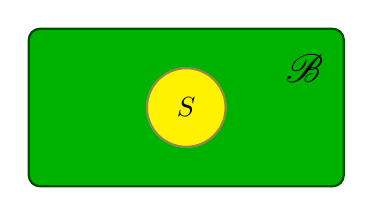
\begin{tikzpicture}
    \filldraw [black!30!green, rounded corners]
            (0,0) rectangle (4,2);
    \filldraw [yellow]
            (2,1) circle (0.5);
    \draw [line width=0.8pt, black!70!green, rounded corners]
            (0,0) rectangle (4,2);
    \draw [line width=0.8pt, black!50!yellow, rounded corners]
            (2,1) circle (0.5);
    \node[text=black] at (3.5,1.5) {\Large{$\bm{\mathscr{B}}$}};
    \node[text=black] at (2,1) {$S$};
    \end{tikzpicture}
    \end{figure}
    \small
    Any empirical test involves a non-negligible influences on the quantum object $ S $ being measured.\\
    $ $\\
    In the approximation of \alertb{weak couplings}, we model the interaction with a Markovian bath $\mathscr{B}$ by the \alert{Lindblad master equation} for the density matrix $\rho$ of the system $S\,$:
    \begin{equation}
    \alert{
    \frac{\partial \rho}{\partial t} = -i \Bigr[ H,\,\rho \Bigr] + \,\D 
    }\,\,.
    \end{equation}
    \end{frame}
    
    %%%%%%%%%%%%%%%%%%%%%%%%%%%%%%%%%%%%%%%%%%%%%%%%%%%%%%%%%%%%%%%%%%%%%%%%%%%%%%%%%%%%%%%%%%%%%%%%%%%%
    
    \begin{frame}
    \frametitle{Open quantum systems}
    %\framesubtitle{Quantum Ising model}
    If $b$ indicates the parts of the open system $S\,$ in contact with an independent bath, the dissipator $\D\,$ corresponds to the sum:
    \[
    \alertb{
    \D = \sum _b w_b\,\D_b} \, \,,\qquad  \alertb{\D_b =  L_b \rho L_b^\dagger - \frac{1}{2}\,\left(\rho L_b^\dagger L_b + L_b^\dagger L_b \rho \right) }\,\, ,
    \]
    where the Lindblad operator $L_b$ describes the interaction of the system part $b$ with its independent environment $\mathscr{B}_{b}$ and $w_b$ tunes the strength of the associated dissipative mechanism.
    
    \begin{figure}[!t]
    \centering
    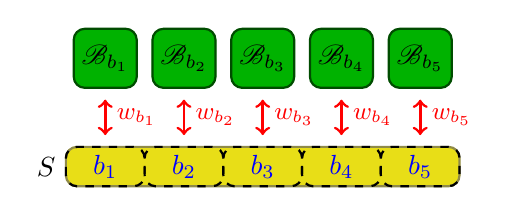
\begin{tikzpicture}
    \filldraw [black!10!yellow, rounded corners]
            (1,-0.25) rectangle (6,0.25);
    \draw [line width=0.8pt, black!50!yellow, rounded corners]
            (1,-0.25) rectangle (6,0.25);
    
        \foreach \i in {1,...,5}
    {
    \filldraw [black!30!green, rounded corners]
            (\i+0.1,1) rectangle (\i+0.9,1.75);
    \draw [line width=0.8pt, black!70!green, rounded corners]
            (\i+0.1,1) rectangle (\i+0.9,1.75);
    \draw [dashed,line width=0.8pt, black, rounded corners]
            (\i,-0.25) rectangle (\i+1,0.25);
    \node[text=black] at (\i+0.5,1.375) {$\mathscr{B}_{b_{\i}}$};
    \node[text=blue] at (\i+0.5,0) {$b_{\i}$};
    
    \draw [<->, line width=1pt,red] (\i+0.5,0.4) -- (\i+0.5,0.85);
    \node[text=red] at (\i+0.9,0.625) {\small{$w_{b_{\i}}$}};
    }
    
    \node[text=black] at (0.75,0) {$S$};
    \end{tikzpicture}
    \end{figure}
    
    \end{frame}



\begin{frame}
\frametitle{Sunburst geometry}

\begin{figure}
    \centering
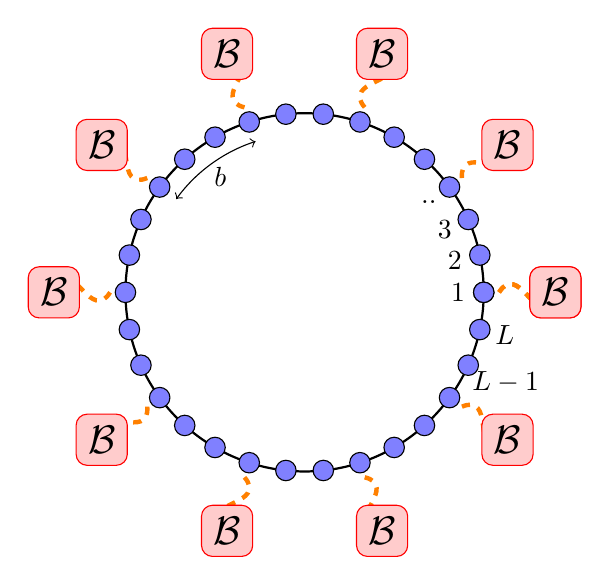
\begin{tikzpicture}[scale=0.65]
    \draw[thick] (0,0) circle (3.5cm);

    \foreach \x in {0,12,...,360}
    \filldraw [fill=blue!50] (\x:3.5cm) circle (0.2);

    \foreach \x in {0,36,...,360}
    \draw[orange, dashed, ultra thick] (\x:3.8cm) .. controls (\x+8:4.2cm) and (\x-8:4.6cm) .. (\x:4.6cm);

    \foreach \x in {0,36,...,360}
    \node[rectangle,
    draw = red,
    text = black,
    fill = red!20!white,
    rounded corners,
    minimum size=0.65cm] (r) at (\x:4.9cm) {\Large $\mathcal{B}$};

    \draw[<->] (108:3.1cm) arc
    [start angle=108,
        end angle=144,
        radius=3.1cm,
    ] ;

    \node[] (s1) at (126:2.8cm) {$b$};

    \node[] (s1) at (0:3cm) {$1$};
    \node[] (s2) at (12:3cm) {$2$};
    \node[] (s3) at (24:3cm) {$3$};
    \node[] (s4) at (36:3cm) {$..$};
    \node[] (s5) at (-12:4cm) {$L$};
    \node[] (s6) at (-24:4.3cm) {$L-1$};
\end{tikzpicture}
    \caption{Sketch of a Kitaev ring with $L=30$ qubits coupled with $n=10$ dissipators in a \textit{sunburst} geometry ($b=3$ in the figure).}
    \label{fig_sketch_sunburst_dissipation}
\end{figure}


\end{frame}


\begin{frame}
	\frametitle{Liouvillian gap}

\ba{eigencalL}
        \widetilde{\cal L}[\widetilde \rho_i] = \lambda_i \widetilde \rho_i \cm
        \qquad \lambda_i \in \numberset{C} \pc
\ea

\be{vecrho}
        \rho_{ij} \ket i \bra j  \longrightarrow  \widetilde \rho_{ij} \ket i \ket j \pt
\ee

\ba{vecteqlindblad}
        \widetilde{\mathcal{L}} =& -i \big(\hat{H} \otimes \hat{\mathbb{I}}
                - \hat{\mathbb{I}}\otimes \hat{H}^t \big) +
                w\sum_{x \in {\cal I}}\hat{L}_{x}\otimes \hat{L}^*_{x}\\
        &-\frac{w}{2}\sum_{x \in {\cal I}}\big(\hat{L}^{\dagger}_{x}\hat{L}_{x}
                \otimes\hat{\mathbb{I}}+\hat{\mathbb{I}}
                        \otimes\hat{L}^t_{x}\hat{L}^*_{x}\big) \pt
\ea

\ba{Lioulliangap}
\Delta_{\lambda} = - \max_{i} {\rm Re}{\lambda_i } \pt
\ea


\end{frame}


\begin{frame}
	\frametitle{Interplay between local and homogeneous dissipation}
	The number of the external baths:
	\be{}
		n \equiv L / b \pc
	\ee
	$ $\\
	\vspace{0.5cm}
	$b$ fixed  $\longrightarrow$ local dissipation with 
	$\Delta_\lambda \sim L^{-1} f(\mu, wL) 
	\qquad L\to\infty \pc$\\
	\vspace{1cm}
	$n$ fixed $\longrightarrow$ homogeneous dissipation with
	$\Delta_\lambda \sim L^{-3} \tilde{f}(\mu, w)
	\qquad L\to\infty\,\,$.
\end{frame}

\begin{frame}
	\frametitle{Liouvillian gap $b$ fixed}
\begin{figure}[!h]
    \centering
    \includegraphics[width=6.4cm]{imm/gapliouv3b.pdf}
	\includegraphics[width=6.4cm]{imm/ratelatetime.pdf}
    \caption{Liouvillian gap $\Delta_\lambda$ in terms of the dissipation coupling $w$ for $b=3$ and fixed $\mu=-2$.}
    \label{fig_liouvgap3b}
\end{figure}
\begin{equation}
    \Delta_\lambda(w, b)=A_\mu(b) w\,,\quad A_\mu(b)=\frac{C_\mu}{b^{3}}\,,\quad w>w_*\,,
    \label{eq_liouvillian_gap_largeL}
\end{equation}
\end{frame}

\begin{frame}
	\frametitle{Liouvillian gap $b$ fixed}
\begin{figure}
    \centering
    \includegraphics[width=8cm]{imm/scalingDeltaapbc.pdf}
    \label{fig_ratelatetime}
\end{figure}

\end{frame}

\begin{frame}
	\frametitle{Liouvillian gap $n$ fixed}
\begin{figure}[!b]
    \centering
    \includegraphics[width=6.4cm]{imm/delantipk0bl2L3Dw.pdf}
    \includegraphics[width=6.4cm]{imm/scalingDeltanfixedmuminus1.pdf}
	\label{fig_scaling_delta_apbc}
\end{figure}

\end{frame}

\begin{frame}
	\frametitle{Dynamic Finite Size Scaling}
	The correlation function as observable:
	\begin{align}
        C(x, y, t)&\equiv{\rm Tr}[\rho(t)(\hat{c}^\dagger_x\hat{c}_y+\hat{c}^\dagger_y\hat{c}_x)]\,,\\
        P(x, y, t)&\equiv{\rm Tr}[\rho(t)(\hat{c}^\dagger_x\hat{c}^\dagger_y+\hat{c}_y\hat{c}_x)]\,.
    \label{eq_def_two_point_functions_C_P}
	\end{align}


	The scaling parameters are set:
	\ba{}
	M_{i/f}=(\mu_{i/f}-\mu_c)L^{y_\mu} &\qquad y_\mu = 1 \pc \\
	\Theta = t L^{-z}\,,\,\, z=1 \,\, 
	{\rm for} \,\, t \sim L &\pc \qquad
	\Theta = t /\Delta_\lambda \,\, 
	{\rm for} \,\, t\sim L^3 \pc \\
	\gamma_b=\frac{wL^{z}}{b}\,& \,\,.
	\ea


	The Scaling Laws can be expressed:
	\begin{align}
    C(x, y, t) &\approx L^{-2y_c}\mathcal{C}(M_i, M_f, \{X_i\}, \Theta, \gamma_b) \,\, ,   \notag \\
    P(x, y, t) &\approx L^{-2y_c}\mathcal{P}(M_i, M_f, \{X_i\}, \Theta, \gamma_b)\,.\notag
\end{align}

\end{frame}

\begin{frame}
	\frametitle{Numerical Results}
	\begin{figure}
    \centering
    \includegraphics[width=6.4cm]{imm/Cscaling2b.pdf}
    \includegraphics[width=6.4cm]{imm/fss_and_gap_n_fixed.pdf}
    \label{fig_Cscaling2b}
\end{figure}
We introduce the RG invariant quantity $R_n$ defined as 
\begin{equation}
    R_n = \frac{N(t) - N_{\text{asy}}}{N(0) - N_{\text{asy}}}\,,
    \label{def_Rn}
\end{equation}
where $N(t)=\sum_x^L\langle\hat c^\dagger_x \hat c_x(t)\rangle$
and $N_{\text{asy}}=\lim_{t\to\infty}N(t)$. 

\end{frame}

   \section{Conclusions}

\begin{frame}
	\frametitle{Conclusions}
	{\bf In the round-trip model:}
	\begin{itemize}
      	\item
      		Analogy of the scaling behaviors at classical and quantum transitions 
      		is only partially extended to round-trip KZ protocols. 
      		Substantial differences emerge:
      		\begin{enumerate} 
      			\item
      				classical systems develop scaling hysteresis-like scenarios, 
      			\item
      				in quantum systems, the persistence of oscillating relative 
      				phases make the return way extremely sensitive to the 
      				parameters of the protocol;
		\end{enumerate}
		
      	\medskip
      	\medskip

      	\item
      		Even in the simple two-level quantum model, we have a similar 
      		behavior.
      \end{itemize}
      
      \medskip
      \medskip
      \medskip
      
      {\bf In the dissipation scenario:}
      \begin{itemize}
      	\item
      		When we keep $b$ fixed, the gap $\Delta_\lambda$ is always finite
      		 and depends linearly on the dissipation strength $w \pc$ 
      	\medskip
      	\medskip
      	\item 			
      		 Two different regimes: 
      		 \begin{enumerate}
      		 	\item In the small $w$ region, the gap is given by 
      		 	$\Delta_\lambda = w/(2b) \pc$

			\item At large $w$ and sufficiently large $b$,
			$\Delta_\lambda = wC_\mu /b^3$ controls the gap
			in the large-size limit and the dynamic FSS.
		\end{enumerate}

      \end{itemize}

\end{frame}


\end{document}
